% mnras_template.tex 
%
% LaTeX template for creating an MNRAS paper
%
% v3.3 released April 2024
% (version numbers match those of mnras.cls)
%
% Copyright (C) Royal Astronomical Society 2015
% Authors:
% Keith T. Smith (Royal Astronomical Society)

% Change log
%
% v3.3 April 2024
%   Updated \pubyear to print the current year automatically
% v3.2 July 2023
%	Updated guidance on use of amssymb package
% v3.0 May 2015
%    Renamed to match the new package name
%    Version number matches mnras.cls
%    A few minor tweaks to wording
% v1.0 September 2013
%    Beta testing only - never publicly released
%    First version: a simple (ish) template for creating an MNRAS paper

%%%%%%%%%%%%%%%%%%%%%%%%%%%%%%%%%%%%%%%%%%%%%%%%%%
% Basic setup. Most papers should leave these options alone.
\documentclass[fleqn,usenatbib]{mnras}

% MNRAS is set in Times font. If you don't have this installed (most LaTeX
% installations will be fine) or prefer the old Computer Modern fonts, comment
% out the following line
\usepackage{newtxtext,newtxmath}
% Depending on your LaTeX fonts installation, you might get better results with one of these:
%\usepackage{mathptmx}
%\usepackage{txfonts}

% Use vector fonts, so it zooms properly in on-screen viewing software
% Don't change these lines unless you know what you are doing
\usepackage[T1]{fontenc}

% Allow "Thomas van Noord" and "Simon de Laguarde" and alike to be sorted by "N" and "L" etc. in the bibliography.
% Write the name in the bibliography as "\VAN{Noord}{Van}{van} Noord, Thomas"
\DeclareRobustCommand{\VAN}[3]{#2}
\let\VANthebibliography\thebibliography
\def\thebibliography{\DeclareRobustCommand{\VAN}[3]{##3}\VANthebibliography}


%%%%% AUTHORS - PLACE YOUR OWN PACKAGES HERE %%%%%

% Only include extra packages if you really need them. Avoid using amssymb if newtxmath is enabled, as these packages can cause conflicts. newtxmatch covers the same math symbols while producing a consistent Times New Roman font. Common packages are:
\usepackage{graphicx}	% Including figure files
\usepackage{amsmath}	% Advanced maths commands

%%%%%%%%%%%%%%%%%%%%%%%%%%%%%%%%%%%%%%%%%%%%%%%%%%

%%%%% AUTHORS - PLACE YOUR OWN COMMANDS HERE %%%%%

% Please keep new commands to a minimum, and use \newcommand not \def to avoid
% overwriting existing commands. Example:
%\newcommand{\pcm}{\,cm$^{-2}$}	% per cm-squared

%%%%%%%%%%%%%%%%%%%%%%%%%%%%%%%%%%%%%%%%%%%%%%%%%%

%%%%%%%%%%%%%%%%%%% TITLE PAGE %%%%%%%%%%%%%%%%%%%

% Title of the paper, and the short title which is used in the headers.
% Keep the title short and informative.
\title[Short title, max. 45 characters]{Velocity Dispersion During the Milky Way Andromeda Merger}

% The list of authors, and the short list which is used in the headers.
% If you need two or more lines of authors, add an extra line using \newauthor
\author[M. J. Lagnado et al.]{
Matan J. Lagnado,$^{1}$\thanks{E-mail: mlagnado@arizona.edu}
\\
% List of institutions
$^{1}$University of Arizona\\
}

% These dates will be filled out by the publisher
\date{Received 04/11/2025}

% Prints the current year, for the copyright statements etc. To achieve a fixed year, replace the expression with a number. 
\pubyear{\the\year{}}

% Don't change these lines
\begin{document}
\label{firstpage}
\pagerange{\pageref{firstpage}--\pageref{lastpage}}
\maketitle


% Select between one and six entries from the list of approved keywords.
% Don't make up new ones.
\begin{keywords}
\textbf{Velocity Dispersion -- Jacobi Radius -- Stellar Disk -- Stellar Bulge -- Local Group}
\end{keywords}

%%%%%%%%%%%%%%%%%%%%%%%%%%%%%%%%%%%%%%%%%%%%%%%%%%

%%%%%%%%%%%%%%%%% BODY OF PAPER %%%%%%%%%%%%%%%%%%

\section{Introduction}

This study looks into how velocity dispersion changes throughout the interaction/collision between the Milky Way (MW) and the Andromeda Galaxy (M31). \textbf{Velocity Dispersion} is the measure of how randomly stars are moving, a smaller dispersion means stars are moving similarly to one another. These two galaxies are in our \textbf{local group}, a collection of many large nearby galaxies as well as the Milky Way's satellite galaxies. During the MW-M31 merger there are many masses interacting with each other, causing changes in trajectories, which in turn cause velocity changes. Understanding how the velocity dispersion changes during the interaction helps both in predicting the resulting galaxy from the merger as well as understanding how mass is distributed.

Understanding how the velocity distribution changes throughout the collision helps us to understand how galaxies evolve when they interact with their neighbors. A \textbf{galaxy} is a gravitationally bound collection of stars whose properties cannot be explained by a combination of baryons and Newton's laws of gravity.\cite{Willman_2012} Various forces, such as gravity, influence the velocity dispersion, which describes a galaxies evolution whether that be structure, density, or size. \textbf{Galaxy evolution} is the process by which a galaxy changes with respect to time, it can be influenced by its stellar population as well as galactic collisions. Developing a better understanding of how velocity dispersion changes within a galaxy during a merger can help us understand how a galaxy might evolve moving forward, and in turn how a galaxy could have evolved to where it is today.

When two galaxies collide, the large disturbance in each of their systems causes a change in stellar movements. The velocity dispersion is a way to measure the movement of stars through a galaxy. When there is a smaller dispersion of velocities in a system it tells us that all the stars are moving in a more ordered pattern, this could explain spiral arms. However, with a greater dispersion the star movement looks more random or chaotic, which is more representative of an elliptical galaxy. When two galaxies merge there are forces that drastically change speeds and directions of where stars are moving, but with each close approach of the two galaxies the stars begin to settle and find a new equilibrium as seen in Figure 1 \cite{Stickley_2012}. These changes can have an effect on the overall structure of the galaxy as well, for example, a high velocity dispersion supports a thickened disk model \cite{Dalcanton_2023}.

\begin{figure}
    \centering
    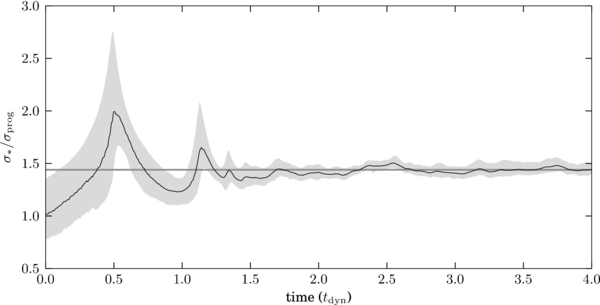
\includegraphics[width=1\linewidth]{Stickley2012.jpg}
    \caption{Shows how velocity dispersion changes throughout a merger. Black line is the mean, with uncertainty within the shaded gray region. The gray line is the final mean value of the dispersion.}\cite{Stickley_2012}
    \label{fig:enter-label}
\end{figure}

Many questions on this topic relate to creating more accurate and higher-resolution models to describe and predict velocity dispersion in galaxies \cite{Han_2024}. To create more accurate models more data is required which is expected of the upcoming completion of the Vera C. Rubin Observatory \cite{refId0}. Following more accurate models higher resolution models can be constructed to consider details such as dust absorption as well as 3D velocity dispersion.

\section{This Project}

In this paper, we will evaluate how the velocity dispersion of each galaxy evolves throughout the MW/M31 interaction. At various important steps during the interaction we will look into how the velocity dispersion changes throughout the galaxy up to its Jacobi Radius. The \textbf{Jacobi Radius} is the radius at which a particle is no longer gravitationally bound to a system. Beyond that radius, particles are no longer bound by a galaxy's gravity. Furthermore, the interesting points during the interaction will be when the two centers of mass are at a local maxima or minima. These points of interest can be compared to the initial velocity dispersion to draw conclusions on galactic evolution throughout the merger.

This project addresses trying to predict galaxy evolution through velocity dispersion with high-resolution models of the merging event.

This question is important to look into because it provides the opportunity to deepen our understanding of galaxy evolution. As we currently understand them, galactic collisions are a driver for stellar evolution. \cite{Schawinski_2010} It can be difficult to measure velocity dispersion of other galaxies due to limited resolution, thus high-resolution simulations can help us draw connections between the snapshots of galaxies we see today. This study will help by analyzing high-resolution simulation to present the evolution of velocity dispersion throughout the MW/M31 interaction.


\section{Methodology}

This simulation utilized in this study is an N-body smoothed-particle hydrodynamics code, GADGET3. \cite{10.1111/j.1365-2966.2005.09655.x} An N-body simulation is a simulation used to model the motion of N individual particles and their gravitational influence on one another. The model incorporates star formation and supernova feedback which is not typically used in  other cosmological simulations. \cite{10.1046/j.1365-8711.2003.06206.x} Each galaxy in this simulation is modeled by three components disk, bulge, and halo. The \textbf{stellar disk} is the flat component of the galaxy where spiral arms may form and young stars are born. The \textbf{stellar bulge} is the bright central region of a galaxy which is usually spherical. The mass of the halo component is inferred based on the total observed mass of the galaxy which is used to define the Hernquist dark matter profile. \cite{10.1111/j.1365-2966.2012.20466.x}

For this study, first, we utilize the low-resolution models produced to develop initial results. Following that, higher resolution models will be used in order to generate more impactful results.

\begin{figure}
    \centering
    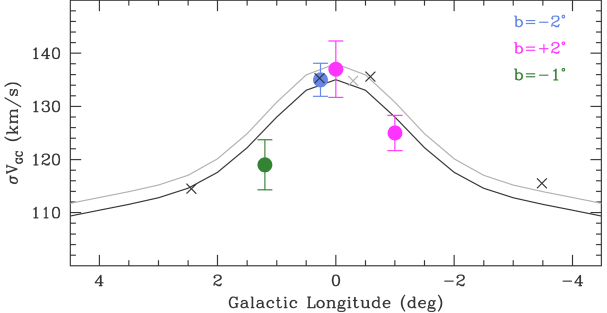
\includegraphics[width=1\linewidth]{Valenti2018.png}
    \caption{Shows how velocity dispersion changes along the longitude of the Milky Way. The solid lines are the expected radial velocity dispersion trends. While the individual points represent observations at various galactic latitude (b).} \cite{refId0}
    \label{fig:enter-label}
\end{figure}

The most important calculation in this question is the velocity dispersion $\sigma$. It can be calculated just like a regular standard deviation, first, calculating the mean velocity and then calculating the squared average deviation from the mean in each coordinate direction:

\begin{equation}
V_{mean} = \frac{1}{N}\sum_{i=1}^Nv_i
\end{equation}
\begin{equation}
\sigma = \sqrt{\frac{1}{N}\sum_{i=1}^N(v_i-V_{mean})^2}
\end{equation}
Where N is the number of particles in one measurement and $v_i$ is the velocity of the ith particle. 
The code will calculate the velocity dispersion of shells of material at constant radii moving outwards until the Jacobi Radius ($R_J$). \cite{1962AJ.....67..471K}
\begin{equation}
    R_J = R(\frac{m}{2M})^{1/3}
\end{equation}
Where $R$ is the separation between the two interacting bodies, m is the mass of the satellite galaxy, and M is the total mass in the system. Only Bulge and Disk type particles will be considered because there isn't an observational way to verify the movement of dark matter particles. The code first slices the galaxy into many spherical shells. Within each of these shells eq. 1 will be used to calculate the mean velocity within of bulge and disk particles. Following that eq. 2 will be used to calculate the velocities dispersion within that shell. This process will be repeated for each minima or maxima for the separation between MW and M31. 


To answer these questions I will need two distinct plots. The first plot simply shows the separation between MW and M31 highlighting the maxima and minima throughout their interaction. Following that, at each of the minima or maxima I will need to produce a plot that displays the velocity dispersion as a function of radius similar to what is done in Figure 2. \cite{refId0} By developing an understanding of how the velocity dispersion changes radially through time we can understand how the shape of a galaxy would change as well. 


Based on the work of Stickley et al. (2012), it is suggested by his N-body simulations that the velocity dispersion increases when a galaxy merger occurs. As Figure 1 shows the final equilibrium of the velocity dispersion increases from the value at $t=0$. I predict that this is happening because of the addition of mass and energy into a system bringing about chaos as the stars attempt to find a new equilibrium. I suspect that following the interaction between the two galaxies the result will be elliptical as the velocity dispersion increases as a whole.

%%%%%%%%%%%%%%%%%%%% REFERENCES %%%%%%%%%%%%%%%%%%

% The best way to enter references is to use BibTeX:

\bibliographystyle{mnras}
\bibliography{example} % if your bibtex file is called example.bib


% Alternatively you could enter them by hand, like this:
% This method is tedious and prone to error if you have lots of references
%\begin{thebibliography}{99}
%\bibitem[\protect\citeauthoryear{Author}{2012}]{Author2012}
%Author A.~N., 2013, Journal of Improbable Astronomy, 1, 1
%\bibitem[\protect\citeauthoryear{Others}{2013}]{Others2013}
%Others S., 2012, Journal of Interesting Stuff, 17, 198
%\end{thebibliography}

%%%%%%%%%%%%%%%%%%%%%%%%%%%%%%%%%%%%%%%%%%%%%%%%%%


% Don't change these lines

\label{lastpage}
\end{document}

% End of mnras_template.tex
